\documentclass{article}

% if you need to pass options to natbib, use, e.g.:
\PassOptionsToPackage{numbers, compress}{natbib}
% before loading neurips_2025

% The authors should use one of these tracks.
% Before accepting by the NeurIPS conference, select one of the options below.
% 0. "default" for submission
%  \usepackage{neurips_2025}
% the "default" option is equal to the "main" option, which is used for the Main Track with double-blind reviewing.
% 1. "main" option is used for the Main Track
%  \usepackage[main]{neurips_2025}
% 2. "position" option is used for the Position Paper Track
%  \usepackage[position]{neurips_2025}
% 3. "dandb" option is used for the Datasets & Benchmarks Track
 % \usepackage[dandb]{neurips_2025}
% 4. "creativeai" option is used for the Creative AI Track
%  \usepackage[creativeai]{neurips_2025}
% 5. "sglblindworkshop" option is used for the Workshop with single-blind reviewing
 % \usepackage[sglblindworkshop]{neurips_2025}
% 6. "dblblindworkshop" option is used for the Workshop with double-blind reviewing
%  \usepackage[dblblindworkshop]{neurips_2025}

% After being accepted, the authors should add "final" behind the track to compile a camera-ready version.
% 1. Main Track
 % \usepackage[main, final]{neurips_2025}
% 2. Position Paper Track
%  \usepackage[position, final]{neurips_2025}
% 3. Datasets & Benchmarks Track
 % \usepackage[dandb, final]{neurips_2025}
% 4. Creative AI Track
%  \usepackage[creativeai, final]{neurips_2025}
% 5. Workshop with single-blind reviewing
%  \usepackage[sglblindworkshop, final]{neurips_2025}
% 6. Workshop with double-blind reviewing
%  \usepackage[dblblindworkshop, final]{neurips_2025}
% Note. For the workshop paper template, both \title{} and \workshoptitle{} are required, with the former indicating the paper title shown in the title and the latter indicating the workshop title displayed in the footnote.
% For workshops (5., 6.), the authors should add the name of the workshop, "\workshoptitle" command is used to set the workshop title.
% \workshoptitle{WORKSHOP TITLE}

% "preprint" option is used for arXiv or other preprint submissions
 \usepackage[preprint]{neurips_2025}

% to avoid loading the natbib package, add option nonatbib:
%    \usepackage[nonatbib]{neurips_2025}

\usepackage[utf8]{inputenc} % allow utf-8 input
\usepackage[T1]{fontenc}    % use 8-bit T1 fonts
\usepackage{hyperref}       % hyperlinks
\usepackage{url}            % simple URL typesetting
\usepackage{booktabs}       % professional-quality tables
\usepackage{amsfonts}       % blackboard math symbols
\usepackage{nicefrac}       % compact symbols for 1/2, etc.
\usepackage{microtype}      % microtypography
\usepackage{xcolor}         % colors
\usepackage{amsmath}
\usepackage{graphicx}
\usepackage{booktabs}
\usepackage{tabularx}
\usepackage{booktabs}
\usepackage{tabularx}
\usepackage{array}
\usepackage{multirow}
\usepackage{makecell}
\usepackage{array} % 用于 \centering 和 \arraybackslash
\usepackage{placeins}

% Note. For the workshop paper template, both \title{} and \workshoptitle{} are required, with the former indicating the paper title shown in the title and the latter indicating the workshop title displayed in the footnote. 
\title{Towards Lightweight Human-Level AI in Trick-Taking Games — An Odyssey in Spades}


% The \author macro works with any number of authors. There are two commands
% used to separate the names and addresses of multiple authors: \And and \AND.
%
% Using \And between authors leaves it to LaTeX to determine where to break the
% lines. Using \AND forces a line break at that point. So, if LaTeX puts 3 of 4
% authors names on the first line, and the last on the second line, try using
% \AND instead of \And before the third author name.


\author{%
  Haoren Luo\thanks{Equal contribution.} \\
  IIIS, Tsinghua University\\
  \texttt{luohr24@mails.tsinghua.edu.cn} \\
  \And
  Bangjie Xu\footnotemark[1] \\
  IIIS, Tsinghua University\\
  \texttt{xbj24@mails.tsinghua.edu.cn} \\
  \And
  Yueyang Wang\footnotemark[1] \\
  IIIS, Tsinghua University\\
  \texttt{wangyuey25@mails.tsinghua.edu.cn} \\
}


\begin{document}


\maketitle


\begin{abstract}
  Developing human-level AI for trick-taking games like Spades is notoriously challenging due to massive imperfect-information state spaces and non-linear scoring dynamics. Pure search methods struggle with combinatorial explosion, while end-to-end deep reinforcement learning often fails to execute precise logical reasoning in the endgame. In this paper, we propose a lightweight, two-stage AI architecture that elegantly bridges these paradigms. We decompose the game into an early phase, handled by a bid-conditional neural policy trained via variance-reduced REINFORCE, and an endgame phase, governed by a highly optimized, sample-based exact solver. Furthermore, we employ Neural Fictitious Self-Play (NFSP) combined with heuristic rules to build a robust bidding model. Evaluations demonstrate that our hybrid approach outperforms traditional search-based and rule-based baselines and achieves human-level performance against skilled human players. Remarkably, our architecture is computationally highly efficient: it executes actions in under 5 seconds on a single CPU core, and the reinforcement learning policy converges in just 20 minutes of training.
\end{abstract}

\section{Introduction}

Spades is a popular trick-taking card game characterized by imperfect information, multi-agent partnership, and complex bidding dynamics. Creating a strong Spades AI is challenging. While purely search-based methods struggle with the large hidden state space, end-to-end Deep Reinforcement Learning (DRL) often suffers from noisy rewards and fails to execute precise logical reasoning in the endgame.

In this paper, we propose a lightweight AI architecture for Spades that achieves strong play without requiring massive computational resources. The system first uses an NFSP-trained bidding MLP to produce the contract, then decomposes card play into two distinct phases. For the early game (the 1st to 4th tricks), we train a Multilayer Perceptron (MLP) using policy-gradient updates, enhanced by careful reward shaping, entropy regularization, and action space restriction. For the endgame (the 5th to 13th tricks), we transition to a sampling-based exact solving approach. By maintaining a probabilistic belief distribution over opponents' hidden hands---derived from their bidding and playing history---we sample the most likely card distributions and evaluate actions using a deterministic Spades exact solver.

The main contributions of this work are three-fold:
\begin{enumerate}
    \item \textbf{Hybrid Two-Stage Architecture:} We introduce an architecture that elegantly bridges model-free RL (for the combinatorially explosive early game) and exact search (for endgame exploitation).
    \item \textbf{Variance-Reduced Team Match Training:} We utilize a duplicate-match reward formulation during REINFORCE training, which evaluates policies on mirrored deals to cancel out the luck of the draw, resulting in highly stable and fast convergence.
    \item \textbf{Bid-Conditional Policy Routing:} We implement a dynamic model-switching mechanism that routes game states to distinct policy networks (Nil vs. Non-Nil) based on the contract, effectively addressing the divergent strategic objectives in Spades.
\end{enumerate}

\begin{figure}[htbp]
    \centering
    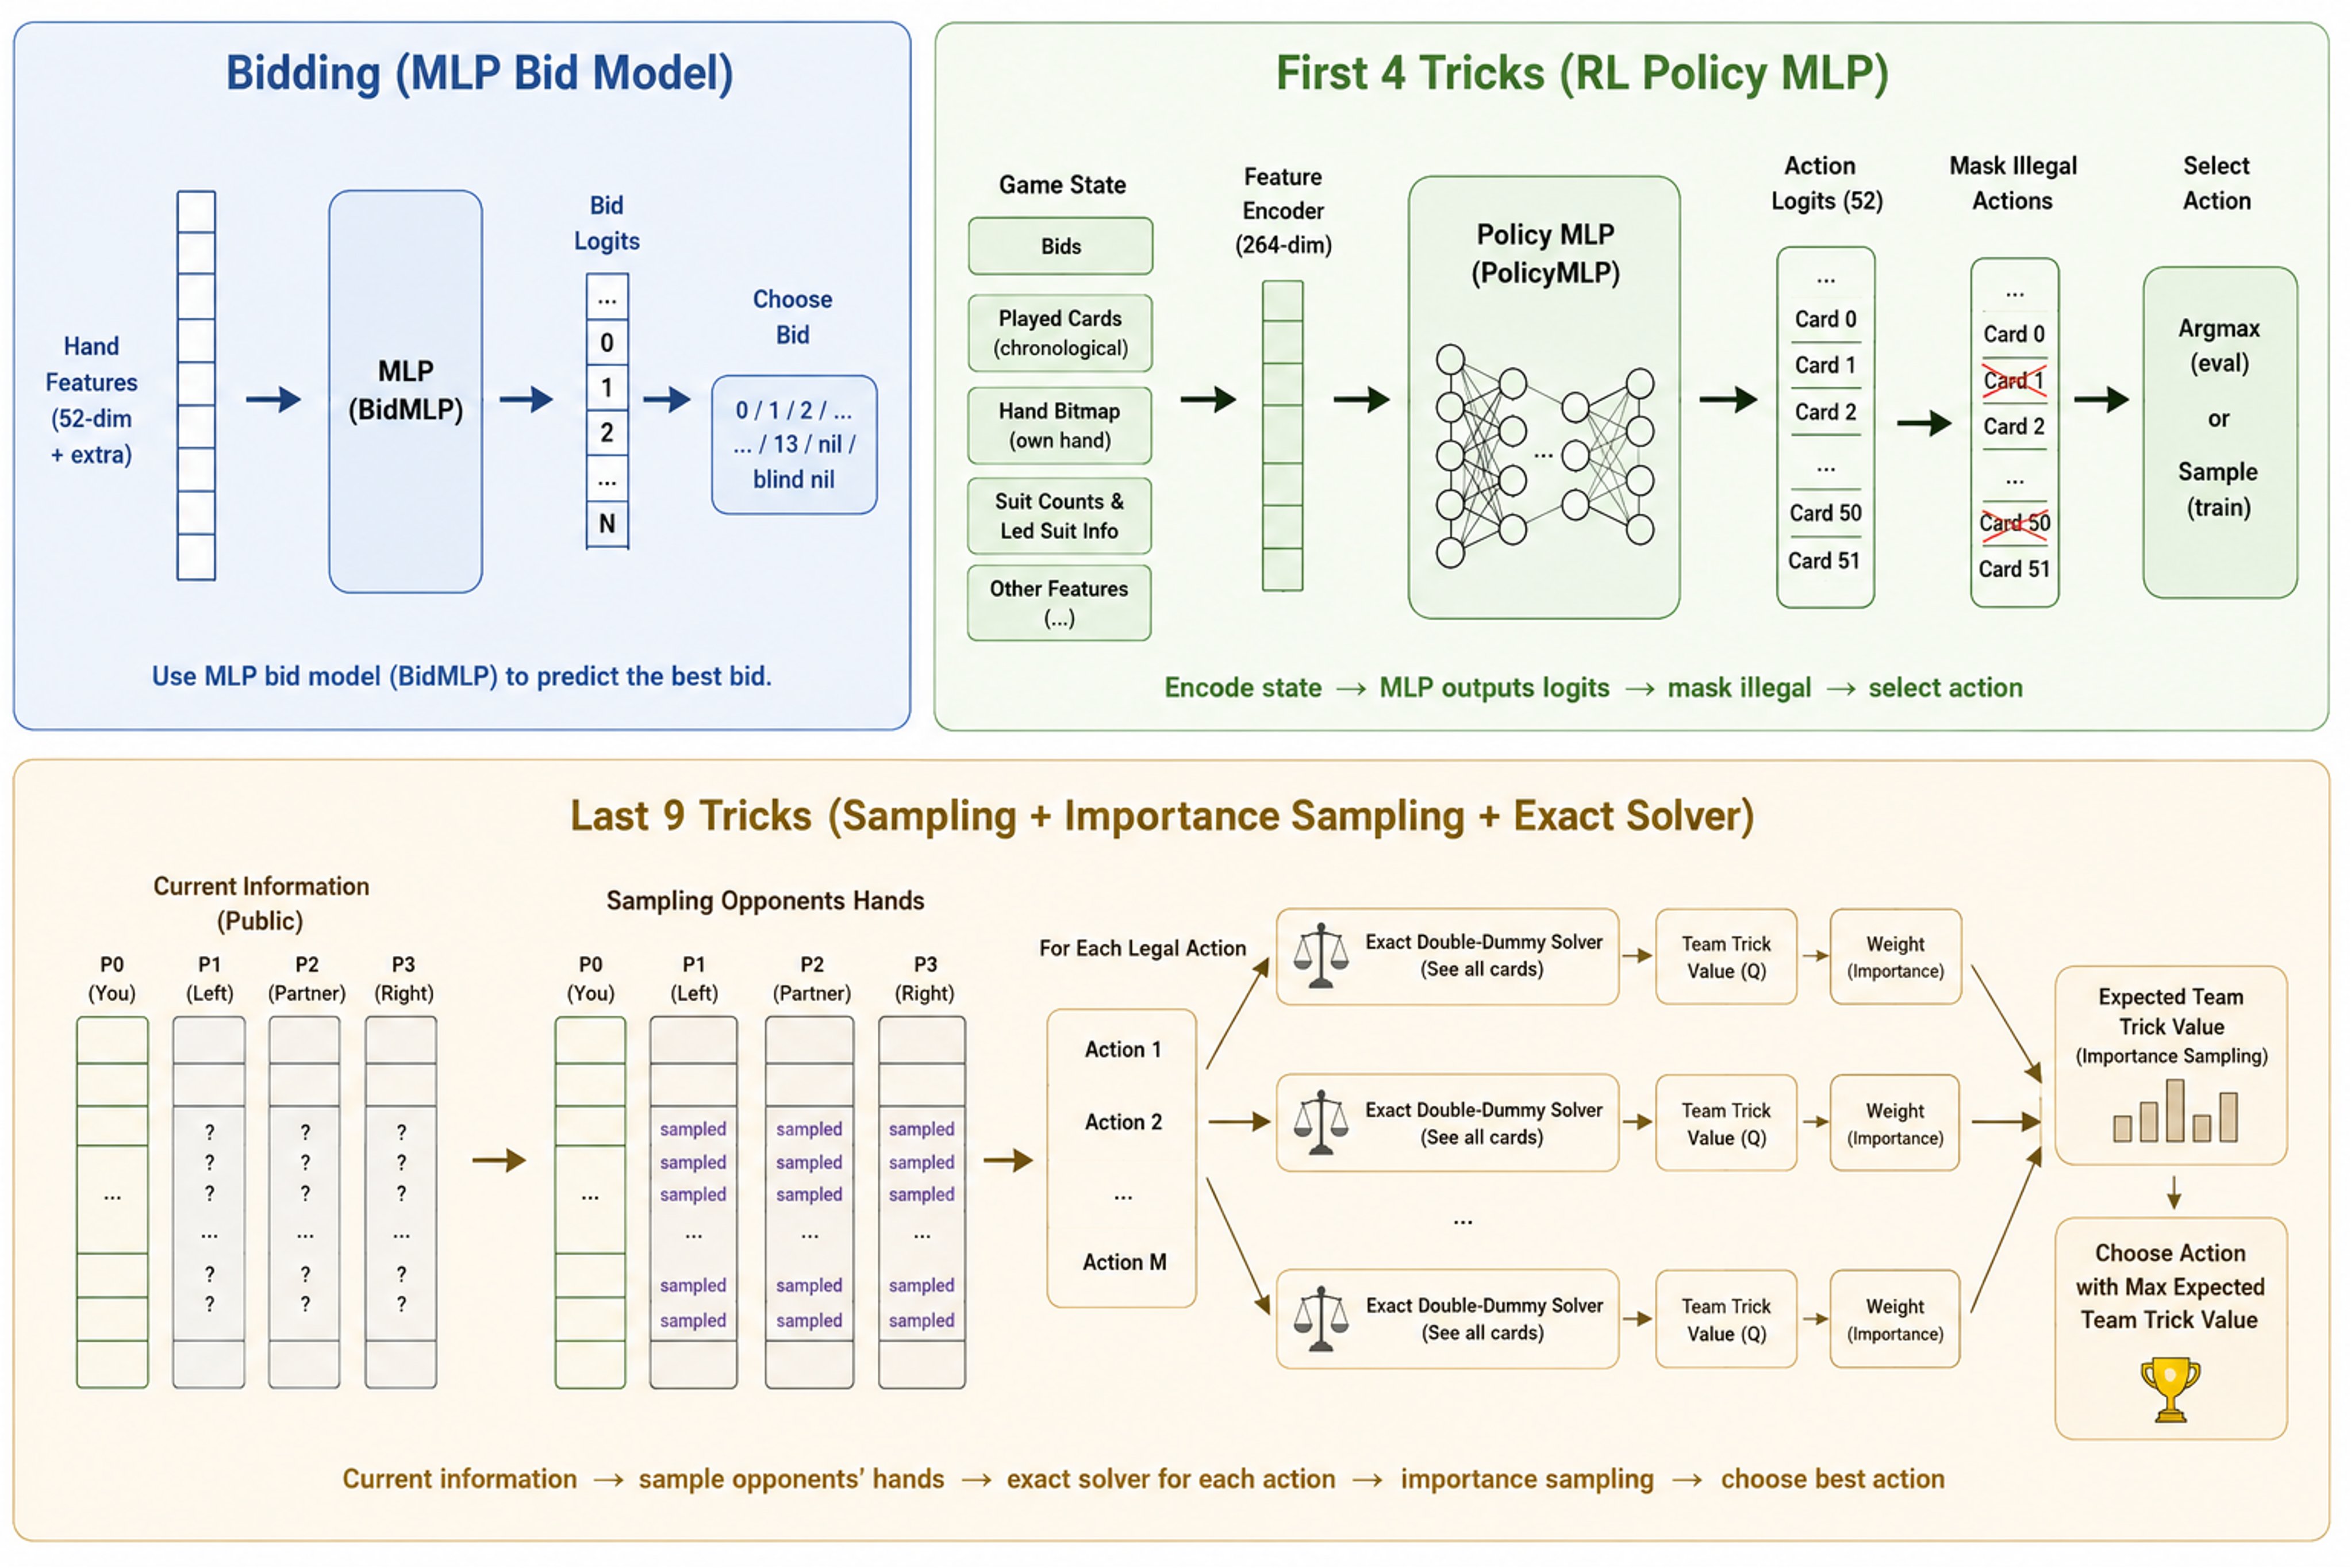
\includegraphics[width=\textwidth]{main_graph.png}
    \caption{Overview of our two-stage AI architecture for Spades.}
    \label{fig:main_graph}
\end{figure}

\section{Preliminaries}

Spades is a four-player, trick-taking card game played in two partnerships. A standard 52-card deck is used, and Spades are the permanent trump suit. The game is characterized by its imperfect information nature and multi-agent cooperation, making it an excellent testbed for AI research. 

A hand of Spades consists of two phases: \textit{bidding} and \textit{playing}. During the bidding phase, players evaluate their 13-card hand and declare the number of tricks they expect to win. A unique feature of Spades is the \textit{Nil} bid, where a player commits to winning exactly zero tricks for a high potential reward or penalty. 

To address the common delay in feedback caused by traditional "bag" penalty rules (where overtricks accumulate across rounds), we adopt a modified \textit{immediate no-bags scoring} rule in this project. In our setting, failing to meet the team's combined bid results in a standard penalty ($-10 \times \mathrm{bid}$), while overtricks are immediately penalized ($-9$ points per overtrick). This forces the AI to bid and play with extreme precision, avoiding the variance of cross-round tracking and providing a denser, more immediate reward signal for reinforcement learning. Detailed rules and scoring mathematics are provided in Appendix \ref{app:rules}.

\textbf{For all the following experiments and training, the objective of each team is to maximize their own team's score minus the opponent team's score, for each single game.}

\section{Related Works}

\paragraph{Frameworks and Environments for Card Game AI.} 
The development of AI for imperfect-information card games has been significantly accelerated by standardized frameworks. \citet{zha2019rlcard} introduced RLCard, a comprehensive toolkit that bridges reinforcement learning with card games, providing standardized environments for games like Blackjack, Texas Hold'em, and Mahjong. More recently, \citet{edelkamp2024framework} proposed a unified framework specifically tailored for general trick-taking card games, encompassing games such as Spades, Hearts, Skat, and Bridge. These environments provide essential infrastructure for evaluating complex algorithms in settings characterized by multi-agent coordination and large, imperfect-information state spaces.

\paragraph{Search and Planning in Imperfect Information Games.} 
Unlike perfect-information games such as Chess or Go, trick-taking games require agents to manage uncertainty regarding opponents' hidden cards. Traditional approaches often rely on Perfect Information Monte Carlo (PIMC) search, which evaluates actions by sampling possible hidden states and averaging the outcomes. However, PIMC suffers from strategy fusion and non-locality issues. To address this, recent work has explored planning directly in the observation space. For example, \citet{gottwald2024transformer} introduced Generative Observation Monte Carlo Tree Search (GO-MCTS), which utilizes a Transformer-based generative model to advance search via observation sequences, demonstrating strong performance in trick-taking games like Hearts and Skat. % Our method shares the spirit of combining learning and search but leverages an exact solver for the endgame to drastically improve accuracy and efficiency.

\paragraph{Exact Solvers and Endgame Analysis.} 
In trick-taking games, as cards are played, the branching factor decreases, allowing for exhaustive search techniques near the end of a round. The Double Dummy Solver (DDS) for Bridge is a prominent example of a highly optimized exact solver operating under perfect information assumptions (when all remaining cards are conceptually revealed) \citep{haglund2024dds}. Inspired by this, our approach integrates an exact Spades solver for the final tricks, using probabilistically sampled hands to approximate the expected Q-values of actions.

\paragraph{Hybrid AI and Learning Beyond Gradients.} 
While pure Deep Reinforcement Learning (DRL) algorithms have achieved superhuman performance in many domains, they often struggle with noisy rewards and sparse feedback in imperfect-information team games. Approaches that integrate knowledge-based systems, heuristics, or search with learning have proven more robust. As discussed in recent perspectives on ``learning beyond gradients'' \citep{weng2026learning_beyond_gradients}, integrating non-differentiable logic---such as restricting the action space using game-theoretic heuristics and performing search-based inference---can significantly accelerate training and stabilize convergence compared to end-to-end policy gradient methods. Our two-stage architecture explicitly adopts this philosophy by combining REINFORCE-based early-trick learning with sample-based exact solving for late-trick reasoning.

\paragraph{Opponent Modeling and Determinization.} 
In multiplayer imperfect-information games, an agent's success heavily depends on predicting the hidden states of other players. Recent advances, such as those discussed at AAAI 2024 \citep{aaai2024opponent}, emphasize explicitly modeling opponent behavior to formulate robust counter-strategies. In games like Spades or Bridge, traditional Perfect Information Monte Carlo (PIMC) methods often use "determinization"---randomly sampling hidden cards that are consistent with the public bidding and playing history. While our approach does not train a complex neural opponent model, we adopt a straightforward and computationally efficient Monte Carlo determinization strategy. By sampling valid opponent hands and feeding them into our exact solver, our AI can approximate optimal endgame plays without the overhead of explicit Bayesian belief tracking.

\section{Bidding}
\label{sec:bidding}

Our deployed bidding strategy is handled by a single NFSP-trained Multi-Layer Perceptron (MLP). In our experiments, the legal bidding space consists of normal bids and \textit{Nil}. Thus \textit{Nil} decisions are made by the same bid model rather than by a separate hard-coded override.

\subsection{MLP Bidding Model}

For the deployed system, all legal bids---including normal bids and \textit{Nil}---come from a trained MLP model. This bidding MLP is a byproduct of the Generative Observation Monte Carlo Tree Search (GO-MCTS) workflow integrated into our Spades AI architecture. The development of this model follows a two-stage training pipeline:
\begin{enumerate}
    \item \textbf{Supervised Learning via DDS:} We first utilize the Double Dummy Solver (DDS) to generate a massive dataset of hands and their exact optimal outcomes under perfect information. This data is used to pre-train two models in a supervised manner: a Transformer model for card playing, and an MLP specifically for bidding.
    \item \textbf{Reinforcement Learning via NFSP:} Because trick-taking games are played under imperfect information, supervised learning on perfect-information targets is insufficient. We therefore apply Neural Fictitious Self-Play (NFSP) to jointly fine-tune the pre-trained playing Transformer and the bidding MLP. Through NFSP reinforcement learning, the bidding MLP adapts its strategy to account for uncertainty and the coordinated nature of the game, resulting in the final bidding model used in our system.
\end{enumerate}

\section{Exact Solver}
\label{sec:exact-solver}

In the late stages of a trick-taking game, the number of possible game states decreases drastically, making it computationally feasible to search for the exact optimal play. Our system integrates a highly optimized Double Dummy Solver (DDS), which computes the game-theoretic value of actions under perfect information (assuming all players' hands are known). The exact solver is framed as a zero-sum game between two teams, utilizing a Minimax algorithm with Alpha-Beta pruning to maximize the score difference between the agent's team and the opposing team.

To support the heavy computational demands required by reasoning through probabilistic sampling (as detailed in Section~\ref{sec:late-game}), our exact solver is engineered in C++ with extreme performance optimizations. It incorporates several advanced search algorithms and domain-specific heuristics:

\begin{enumerate}
    \item \textbf{State Normalization and Transposition Tables}: We utilize Zobrist hashing alongside a large Transposition Table (TT) to cache exact values and alpha/beta bounds. Crucially, we apply Rank Canonicalization (State Normalization), mapping structurally equivalent card distributions (i.e., hands differing only by missing intermediate ranks) to the same hash. This collapses the state space and significantly increases TT hit rates.
    \item \textbf{Equivalent Card Filtering}: The solver identifies equivalent adjacent cards held by a player (e.g., holding both King and Queen of a suit when the Ace is unplayed). By considering only one card from such equivalent sets, the branching factor is heavily reduced.
    \item \textbf{Quick Tricks Pruning}: The solver analyzes guaranteed tricks a player can secure unconditionally (e.g., holding consecutive top trumps). This provides tight lower bounds for early pruning without full expansion.
    \item \textbf{Advanced Search Enhancements}: We further accelerate the solver using Principal Variation Search (PVS) with zero-window searches, Killer Move and History Heuristics for move ordering, and Memory-enhanced Test Driver (MTD(f)) to iteratively converge to the minimax value
\end{enumerate}

By employing these low-level optimizations, avoiding expensive heap allocations during search, and bypassing Python overhead, the exact solver can evaluate endgame branches in microseconds. This makes it a robust and highly efficient engine for the late-trick sampling framework.

\section{Playing}
\label{sec:playing}

\subsection{The 1st to 4th Trick}
\label{sec:early-game}

For the first to fourth trick, we trained an MLP using policy-gradient updates. The deployed model uses a 264-dimensional public-information feature vector and a $264\to 1024\to 512\to 512\to 55$ architecture. The 55 outputs correspond to 52 card logits when leading and three compressed strategic options when following suit.

There are three major designs that make the model work better:

\begin{enumerate}


\item We separately train two models, one for the games in which at least one player bids nil, one for the other situations.

\item End to end training causes great noise in reward. So we manually designed reward shaping (and the rewards are different for the two models). The training time is only 20 minutes.

\item For those actions that are not leading tricks, we restrict the action space size to 3 (the largest card, the smallest card, and the smallest card largest than the cards on the table). This increases gradient update frequencies for the parameters, making training converge faster.


\end{enumerate}

We also add an entropy reward during training to prevent the policy from collapsing. The final system uses two policies with this architecture: a non-Nil model and a Nil-conditional model selected after bidding.

\subsection{The 5th to 13th Trick: Reasoning By Sampling}
\label{sec:late-game}

We used a sampling then exact solving approach. The player needs to sample the opponents' hands since those cards are not revealed, and more accurate sampling leads to better performance.

First, randomly draw 6789 hands. Then calculate each hand's probability:

$$P_i=\prod_{n=1}^4 p_{bid,n} \prod_{t=1}^T p(a_t|s_t)$$

where $p_{bid,i}$ are calculated by the bidding model, and $p(a_t|s_t)$ is 0 if the action is illegal.

We pick the top-$K$ ($K=32$ in the deployed system) hands with the highest $P$ and normalize their weights. An action $a$'s Q-value is $\sum_{i=1}^K P_iQ(a,\textrm{hand }i)$ as an approximation of the action's actual expected Q-value, where $Q(a,\textrm{hand }i)$ are returned by our Spades exact solver. Then, we pick

$$a^* = \arg \max_a \sum_{i=1}^K P_iQ(a,\textrm{hand }i)$$

This is a way which automatically deduces the remaining hands of the other players. Sometimes the hands have special properties, and our model can "reason".

We tried a variety of approaches in calculating $p(a_t\mid s_t)$, but found that all the modifications had little effect on the model's performance. The deployed implementation therefore uses the simplest public-history legality filter: if $a_t$ is legal under $s_t$, $p(a_t\mid s_t)=1$, otherwise $p(a_t\mid s_t)=0$. %A small random jitter is applied only to break degeneracies among nearly identical proposals.


	
\section{Experiments}

\subsection{Baselines}

We benchmark our system against four baselines that span the spectrum from hand-written heuristics to perfect-information search and human play. The two rule-based agents share an identical card abstraction and game interface, differing only in how their heuristics were obtained, which lets us isolate the effect of automated heuristic refinement.

\paragraph{Rule-Based Player 1 (LLM one-shot heuristics).}
Our first baseline is a fully deterministic, rule-based agent written entirely by an LLM coding agent (Claude-Code) in a single ``one-shot'' pass, with no human authoring or hand-tuning of the heuristics. The agent uses no learning and no search, providing a transparent, reproducible lower bound and a fixed starting point for the heuristic-learning baseline below. %Its bidding combines an additive trick-counting heuristic---awarding fractional trick credit to high cards, long trump holdings, and short side suits---with simple partner- and opponent-aware adjustments. Its card play follows a fixed priority list for leading (cash side-suit masters, develop long suits, trump when broken) and following (win when the partnership needs the trick, otherwise duck cheaply). 



\paragraph{Rule-Based Player 2 (LLM heuristic learning).}
Our second baseline starts from Player 1 and is refined by Claude-Code following the \emph{learning beyond gradients} paradigm \citep{weng2026learning_beyond_gradients}, in which a coding agent improves an explicit symbolic policy through a closed feedback loop rather than gradient descent. Each iteration mines counterfactual replays of completed deals (``what score would result had the agent bid or played differently?''), proposes a candidate rule, encodes it as a test-driven patch, and validates it on a large batch of \textit{duplicate} (mirrored) team matches; a patch is committed to a ledger only if it yields a statistically robust positive score margin, and is otherwise rolled back. The guiding constraint is that every accepted change must be supported by counterfactual evidence rather than human intuition. Over a campaign of $22$ logged trials spanning three days, seven patches were accepted into the final policy, raising the per-board score margin over Player 1 from $+0.66$ to $+35.4$ points on $1{,}000$-board duplicate evaluations.

\paragraph{Bridge DDS (perfect-information trick maximizer).}
To quantify the value of optimizing for the true Spades score rather than raw trick count, we include a baseline built on the open-source Bridge Double Dummy Solver \citep{haglund2024dds}, an Apache-2.0 C++ engine that uses alpha--beta search with transposition tables to compute, under perfect information, the line of play that \emph{maximizes the number of tricks won}. We let this player cheat and see opponents' hidden hands, query the Bridge DDS for the trick-maximizing action. Because it greedily chases tricks, it neither protects friendly \textit{Nil} contracts nor avoids immediate overtrick penalties; the resulting search-cost trade-offs are analyzed in detail in Table~\ref{table:solver-comparison}.

\paragraph{Human.}
Two human players of considerable skill, each with at least 100 hours of Spades experience.

\subsection{Bidding Distribution Sanity Check}

To validate that the NFSP-trained bidding model produces globally reasonable contracts, we sampled $10{,}000$ random deals and let the four players bid sequentially using the current bidding logic. We then recorded the sum of the four individual bids, treating \textit{Nil} as $0$. The resulting distribution is shown in Table~\ref{tab:bid-sum-distribution}.

\begin{table}[!htbp]
\centering
\caption{Distribution of the total bid over four players on $10{,}000$ random deals.}
\label{tab:bid-sum-distribution}
\small
\begin{tabular}{crr}
\toprule
\textbf{Total Bid} & \textbf{Count} & \textbf{Percentage} \\
\midrule
7  & 3     & 0.03\% \\
8  & 92    & 0.92\% \\
9  & 867   & 8.67\% \\
10 & 3,774 & 37.74\% \\
11 & 4,103 & 41.03\% \\
12 & 1,050 & 10.50\% \\
13 & 102   & 1.02\% \\
14 & 8     & 0.08\% \\
15 & 1     & 0.01\% \\
\bottomrule
\end{tabular}
\end{table}

The total bid is highly concentrated around $10$--$11$ tricks, with mean $10.55$ and standard deviation $0.87$. This matches common human understanding of Spades bidding: because of uncertainty, partnership coordination, and the penalty for overbidding, rational players usually bid conservatively rather than forcing the total table contract to $13$. In addition, human experts manually inspected the model's bids and judged more than $90\%$ of them to be reasonable, providing further evidence that the bidding model captures human-like contract estimation.
\FloatBarrier

\subsection{Play Of Hand Results}

In the following experiments, the bidding models are the same, so the only difference is the strategy after bidding. For all of the following experiments, we apply a form of match play which is widely used in Bridge competitions. Denote the first, second, third, fourth bidding player as player $0,1,2,3$. If the two methods compared are $A$ and $B$, each deal is played twice, for the first time, players $0,2$ are $A$, players $1,3$ are $B$; for the second time, players $0,2$ are $B$, players $1,3$ are $A$. This greatly reduces variations.

$X \overset{k}{>} Y$  means when two $X$ play against two $Y$,
it is expected that $X$ can earn $k$ more score than $Y$ per game. 

"Cheating" baselines means that the hands of the opponents are revealed to the model, so no sampling is needed. For cheating MCTS-Exact and cheating Bridge DDS, during the whole play, the models are informed of the hands, while for cheating RL-Exact, for the first 4 tricks, the models are not informed of the hands.

\begin{table}[!htbp]
\centering
\small
\caption{Description of the methods}
\label{tab:example}
\begin{tabularx}{\textwidth}{
  >{\centering\arraybackslash}X
  >{\centering\arraybackslash}X
  >{\centering\arraybackslash}X
  >{\centering\arraybackslash}X
  >{\centering\arraybackslash}X
  >{\centering\arraybackslash}X
}
\toprule
\textbf{Name} & 
\textbf{Cheat in the first 4 tricks} & 
\textbf{Cheat in the last 9 tricks} & 
\textbf{Strategy of the first 4 tricks} & 
\textbf{Strategy of the last 9 tricks} & 
\textbf{Bidding} \\
\midrule
Cheating RL-Exact   & No  & Yes & RL-trained MLP             & Spades Solver & \makecell{NFSP\\BidMLP} \\
Cheating MCTS-Exact & Yes & Yes & MCTS                 & Spades Solver & \makecell{NFSP\\BidMLP} \\
Cheating Bridge DDS & Yes & Yes & Bridge Solver        & Bridge Solver & \makecell{NFSP\\BidMLP} \\
RL-Exact            & No  & No  & RL-trained MLP             & Sample Then Spades Solver & \makecell{NFSP\\BidMLP} \\
MCTS-Exact          & No  & No  & Sample Then MCTS     & Sample Then Spades Solver & \makecell{NFSP\\BidMLP} \\
Rule-Based 2        & No  & No  & Rule-Based Player 2  & Rule-Based Player 2 & \makecell{NFSP\\BidMLP} \\
Rule-Based 1        & No  & No  & Rule-Based Player 1  & Rule-Based Player 1 & \makecell{NFSP\\BidMLP} \\
Human             & No  & No  & /  & / & Human bidding \\
\bottomrule
\end{tabularx}
\end{table}
\FloatBarrier


\begin{figure}[htbp]
    \centering
    \begin{minipage}{0.40\textwidth}
        \centering
        \includegraphics[width=1.0\textwidth]{eval_results.png}
        \caption{Evaluation results}
        \label{fig:eval_results}
    \end{minipage}
    \hfill
    \begin{minipage}{0.59\textwidth}
        \centering
        \includegraphics[width=1.0\textwidth]{19_2.png}
        \caption{Detailed Results when our RL-Exact plays against     Rule-Based Player 2}
        \label{fig:rl_vs_rule}
    \end{minipage}
\end{figure}




% \begin{figure}[!htbp]
    
% \end{figure}
% \FloatBarrier

Figure~\ref{fig:eval_results} reports that among the four no-cheating methods, our RL-Exact method is the best.


% \begin{figure}[!htbp]
    
% \end{figure}
% \FloatBarrier

Figure~\ref{fig:rl_vs_rule} reports the head-to-head experiment where our RL-Exact method plays against Rule-Based Player 2. In only 5.75\% of the deals did our method fail to meet the target number of tricks, while the Rule-Based Player 2 failed in 12\% of the deals. Our method succeeded in 79.63\% of nil contracts, whereas the Rule-Based Player 2 had a success rate of only 55.56\%. After manual evaluation of the play, our model demonstrated notable control, offensive and defensive capabilities, and coordination between partners.
\FloatBarrier


\subsection{Overall Results When Competing With Human}

For our RL-Exact AI with the NFSP bidding model, we held three manual matches involving human players with a total of 23 games, as shown in Table~\ref{tab:bridge}. The average score difference was Human - AI = 5.39. Because the sample size is small and the matches were conducted manually, this result should be interpreted as evidence that the AI is competitive with skilled human players rather than as a statistically conclusive human-level claim. Qualitatively, the model consistently exerted pressure on the human players throughout the game, complicating their situational assessment and inducing mistakes.


\begin{table}[!htbp]
\centering
\caption{Match results: total and per‑board scores (our side : opponents)}
\label{tab:bridge}
\small
\begin{tabular}{lcc}
\toprule
\textbf{Setting} & \textbf{Total Score} & \textbf{Per‑Board Scores} \\
\midrule
2 Humans vs 2 AIs
    & 241 : 213
    & 41:70, 82:22, 23:-60, 12:80, 42:50, 41:51 \\
\addlinespace
1 Human+1 AI vs 2 AIs (match 1)
    & 541 : 506
    & \begin{tabular}{@{}l@{}}
        61:12, 2:90, 21:90, 20:53, 70:53, 51:-28, \\
        100:11, 42:50, 60:32, 31:61, 61:12, 22:70
      \end{tabular} \\
\addlinespace
1 Human+1 AI vs 2 AIs (match 2)
    & 257 : 196
    & 62:80, 2:71, 70:-16, 62:30, 61:31 \\
\bottomrule
\end{tabular}
\end{table}
\FloatBarrier

\subsection{Comparison with MCTS}

We also implemented a MCTS baseline which necessitates sampling, causing instability and requiring strong test-time scaling. Our method surpasses the MCTS baseline in both performance and speed (Table~\ref{table:mcts-comparison}). All the bidding models are the NFSP model, and both MCTS and RL use a sample-then-exact strategy in the last 9 tricks.

\begin{table}[!htbp]
  \caption{Performance comparison of MCTS and RL. The bidding and the strategy of the last 9 tricks are the same}
  \label{table:mcts-comparison}
  \centering
  \begin{tabular}{ccc}
    \toprule
    Metrics & MCTS & RL \\
    \midrule
    Average Time Per Action & 10s & <0.1s \\
    Average profit when playing against RL/MCTS & -3.21 & +3.21 \\
    Average profit when playing against Rule Based 2 & +18.59 & +19.27 \\
    \bottomrule
  \end{tabular}
\end{table}
\FloatBarrier

\subsection{Exact Solver vs. Traditional DDS}

A fundamental distinction of our work is the development of an exact solver explicitly tailored for Spades' highly non-linear scoring system. Traditional Double Dummy Solvers (DDS) designed for Bridge solely optimize to maximize the number of tricks won. In Spades, greedy trick maximization is profoundly sub-optimal due to mechanisms like Nil bids (where winning a trick breaks the bid and incurs a severe penalty) and immediate overtrick penalties. Our solver accurately evaluates terminal states using the true Spades score difference, ensuring it protects friendly Nil bids and intentionally avoids overtricks when necessary.

To quantify the computational trade-offs of optimizing for a non-linear score versus a linear trick count, we benchmarked our custom C++ Spades exact solver against a highly optimized Bridge DDS. We evaluated both solvers on 1,000 randomly generated game states at varying depths (remaining cards).

\begin{table}[!htbp]
  \caption{Performance comparison of Bridge DDS vs. our Spades Exact Solver over 1,000 deals.}
  \label{table:solver-comparison}
  \centering
  \begin{tabular}{crrc}
    \toprule
    Remaining Cards & Bridge DDS (ms) & Spades Exact Solver (ms) & Speed Ratio \\
    \midrule
    4 & 0.051 & 0.019 & 0.38x \\
    8 & 0.198 & 0.013 & 0.07x \\
    12 & 0.210 & 0.024 & 0.11x \\
    16 & 0.225 & 0.067 & 0.30x \\
    20 & 0.261 & 0.329 & 1.26x \\
    24 & 0.396 & 1.197 & 3.03x \\
    28 & 0.524 & 4.741 & 9.05x \\
    32 & 0.911 & 25.636 & 28.14x \\
    36 & 1.811 & 238.202 & 131.55x \\
    \bottomrule
  \end{tabular}
\end{table}

As shown in Table~\ref{table:solver-comparison}, as the number of remaining cards increases, our Spades exact solver inevitably scales worse than Bridge DDS (e.g., 238.2ms vs 1.8ms at 36 cards). This exponential divergence is fundamentally theoretical: Bridge DDS benefits from massive algorithmic pruning based on absolute trick certainty (e.g., holding top trumps guarantees winning the trick, allowing entire subtrees to be skipped). In contrast, the highly non-linear Spades objective forces our solver to explore vastly more branches to verify if taking a "guaranteed" trick might actually decrease the overall score via overtrick or Nil penalties. Despite this overhead, our C++ optimizations (such as rank canonicalization and zero-allocation transposition tables) keep the exact solver viable in practice. At our operational threshold of 36 remaining cards, the solver completes a full perfect-information evaluation in roughly 238ms before sampling overhead. This performance is sufficient to run sampled inferences per decision, enabling late-game reasoning without bottlenecking real-time play.

When deployed with 6,789 proposal hands and 32 exact-solved determinizations, the total sampling-and-solving latency remains within interactive play for the last 9 tricks on CPU.

\section{Limitations}

While our two-stage architecture is efficient and competitive, several limitations remain. First, our hand-sampling mechanism for the exact solver relies on a simple public-history legality model plus bid likelihoods. While we explored various modifications, we have yet to discover a more sophisticated sampling technique that consistently improves overall performance, indicating that better modeling of human psychology and specific play styles remains an open challenge. Second, the transition between the early-game RL model and the endgame exact solver is currently hard-coded at the fifth trick (36 remaining cards). This boundary is dictated by the exponential computational scaling of the exact solver; extending the exact search to earlier stages is too slow for real-time play. Third, the human evaluation is small and manual, so it should be treated as qualitative evidence rather than a statistically significant benchmark. Fourth, parts of the RL training pipeline use shaped surrogate rewards rather than the exact final Spades score; this was useful for fast convergence but may bias the policy toward the handcrafted shaping terms. Finally, although the deployed BidMLP can predict \textit{Nil} directly, its risk calibration is still evaluated only indirectly through game outcomes. A more explicit, uncertainty-aware \textit{Nil} calibration study could help the AI discover more nuanced \textit{Nil} opportunities while avoiding unsafe ones.

\section{Conclusion}

In this paper, we presented a lightweight, two-stage AI architecture for Spades that bridges the gap between deep reinforcement learning and exact search. By decomposing the game into a computationally intractable early phase---handled by a fast, bid-conditional MLP trained via variance-reduced policy-gradient updates---and a constrained endgame---solved by a highly optimized, sample-based Spades exact solver---our agent achieves strong play without massive computational resources. Our evaluations show that this hybrid approach outperforms rule-based heuristics, perfect-information trick maximizers, and traditional MCTS baselines under our duplicate-match protocol, while remaining efficient enough for interactive CPU play. Ultimately, our work supports the efficacy of combining neural approximation with explicit symbolic reasoning, offering a practical blueprint for complex, imperfect-information, and multi-agent trick-taking games.

\iffalse % === COMMENTED OUT FORMATTING INSTRUCTIONS ===
Papers to be submitted to NeurIPS 2025 must be prepared according to the
instructions presented here. Papers may only be up to {\bf nine} pages long,
including figures.
% Additional pages \emph{containing only acknowledgments and references} are allowed.
Additional pages \emph{containing references, checklist, and the optional technical appendices} do not count as content pages.
Papers that exceed the page limit will not be
reviewed, or in any other way considered for presentation at the conference.


The margins in 2025 are the same as those in previous years.


Authors are required to use the NeurIPS \LaTeX{} style files obtainable at the
NeurIPS website as indicated below. Please make sure you use the current files
and not previous versions. Tweaking the style files may be grounds for
rejection.


\subsection{Retrieval of style files}


The style files for NeurIPS and other conference information are available on
the website at
\begin{center}
  \url{https://neurips.cc}
\end{center}
The file \verb+neurips_2025.pdf+ contains these instructions and illustrates the
various formatting requirements your NeurIPS paper must satisfy.


The only supported style file for NeurIPS 2025 is \verb+neurips_2025.sty+,
rewritten for \LaTeXe{}.  \textbf{Previous style files for \LaTeX{} 2.09,
  Microsoft Word, and RTF are no longer supported!}


The \LaTeX{} style file contains three optional arguments: \verb+final+, which
creates a camera-ready copy, \verb+preprint+, which creates a preprint for
submission to, e.g., arXiv, and \verb+nonatbib+, which will not load the
\verb+natbib+ package for you in case of package clash.


\paragraph{Preprint option}
If you wish to post a preprint of your work online, e.g., on arXiv, using the
NeurIPS style, please use the \verb+preprint+ option. This will create a
nonanonymized version of your work with the text ``Preprint. Work in progress.''
in the footer. This version may be distributed as you see fit, as long as you do not say which conference it was submitted to. Please \textbf{do
  not} use the \verb+final+ option, which should \textbf{only} be used for
papers accepted to NeurIPS.


At submission time, please omit the \verb+final+ and \verb+preprint+
options. This will anonymize your submission and add line numbers to aid
review. Please do \emph{not} refer to these line numbers in your paper as they
will be removed during generation of camera-ready copies.


The file \verb+neurips_2025.tex+ may be used as a ``shell'' for writing your
paper. All you have to do is replace the author, title, abstract, and text of
the paper with your own.


The formatting instructions contained in these style files are summarized in
Sections \ref{gen_inst}, \ref{headings}, and \ref{others} below.


\section{General formatting instructions}
\label{gen_inst}


The text must be confined within a rectangle 5.5~inches (33~picas) wide and
9~inches (54~picas) long. The left margin is 1.5~inch (9~picas).  Use 10~point
type with a vertical spacing (leading) of 11~points.  Times New Roman is the
preferred typeface throughout, and will be selected for you by default.
Paragraphs are separated by \nicefrac{1}{2}~line space (5.5 points), with no
indentation.


The paper title should be 17~point, initial caps/lower case, bold, centered
between two horizontal rules. The top rule should be 4~points thick and the
bottom rule should be 1~point thick. Allow \nicefrac{1}{4}~inch space above and
below the title to rules. All pages should start at 1~inch (6~picas) from the
top of the page.


For the final version, authors' names are set in boldface, and each name is
centered above the corresponding address. The lead author's name is to be listed
first (left-most), and the co-authors' names (if different address) are set to
follow. If there is only one co-author, list both author and co-author side by
side.


Please pay special attention to the instructions in Section \ref{others}
regarding figures, tables, acknowledgments, and references.

\section{Headings: first level}
\label{headings}


All headings should be lower case (except for first word and proper nouns),
flush left, and bold.


First-level headings should be in 12-point type.


\subsection{Headings: second level}


Second-level headings should be in 10-point type.


\subsubsection{Headings: third level}


Third-level headings should be in 10-point type.


\paragraph{Paragraphs}


There is also a \verb+\paragraph+ command available, which sets the heading in
bold, flush left, and inline with the text, with the heading followed by 1\,em
of space.


\section{Citations, figures, tables, references}
\label{others}


These instructions apply to everyone.


\subsection{Citations within the text}


The \verb+natbib+ package will be loaded for you by default.  Citations may be
author/year or numeric, as long as you maintain internal consistency.  As to the
format of the references themselves, any style is acceptable as long as it is
used consistently.


The documentation for \verb+natbib+ may be found at
\begin{center}
  \url{http://mirrors.ctan.org/macros/latex/contrib/natbib/natnotes.pdf}
\end{center}
Of note is the command \verb+\citet+, which produces citations appropriate for
use in inline text.  For example,
\begin{verbatim}
   \citet{hasselmo} investigated\dots
\end{verbatim}
produces
\begin{quote}
  Hasselmo, et al.\ (1995) investigated\dots
\end{quote}


If you wish to load the \verb+natbib+ package with options, you may add the
following before loading the \verb+neurips_2025+ package:
\begin{verbatim}
   \PassOptionsToPackage{options}{natbib}
\end{verbatim}


If \verb+natbib+ clashes with another package you load, you can add the optional
argument \verb+nonatbib+ when loading the style file:
\begin{verbatim}
   \usepackage[nonatbib]{neurips_2025}
\end{verbatim}


As submission is double blind, refer to your own published work in the third
person. That is, use ``In the previous work of Jones et al.\ [4],'' not ``In our
previous work [4].'' If you cite your other papers that are not widely available
(e.g., a journal paper under review), use anonymous author names in the
citation, e.g., an author of the form ``A.\ Anonymous'' and include a copy of the anonymized paper in the supplementary material.


\subsection{Footnotes}


Footnotes should be used sparingly.  If you do require a footnote, indicate
footnotes with a number\footnote{Sample of the first footnote.} in the
text. Place the footnotes at the bottom of the page on which they appear.
Precede the footnote with a horizontal rule of 2~inches (12~picas).


Note that footnotes are properly typeset \emph{after} punctuation
marks.\footnote{As in this example.}


\subsection{Figures}


\begin{figure}
  \centering
  \fbox{\rule[-.5cm]{0cm}{4cm} \rule[-.5cm]{4cm}{0cm}}
  \caption{Sample figure caption.}
\end{figure}


All artwork must be neat, clean, and legible. Lines should be dark enough for
purposes of reproduction. The figure number and caption always appear after the
figure. Place one line space before the figure caption and one line space after
the figure. The figure caption should be lower case (except for first word and
proper nouns); figures are numbered consecutively.


You may use color figures.  However, it is best for the figure captions and the
paper body to be legible if the paper is printed in either black/white or in
color.


\subsection{Tables}


All tables must be centered, neat, clean and legible.  The table number and
title always appear before the table.  See Table~\ref{sample-table}.


Place one line space before the table title, one line space after the
table title, and one line space after the table. The table title must
be lower case (except for first word and proper nouns); tables are
numbered consecutively.


Note that publication-quality tables \emph{do not contain vertical rules.} We
strongly suggest the use of the \verb+booktabs+ package, which allows for
typesetting high-quality, professional tables:
\begin{center}
  \url{https://www.ctan.org/pkg/booktabs}
\end{center}
This package was used to typeset Table~\ref{sample-table}.


\begin{table}
  \caption{Sample table title}
  \label{sample-table}
  \centering
  \begin{tabular}{lll}
    \toprule
    \multicolumn{2}{c}{Part}                   \\
    \cmidrule(r){1-2}
    Name     & Description     & Size ($\mu$m) \\
    \midrule
    Dendrite & Input terminal  & $\sim$100     \\
    Axon     & Output terminal & $\sim$10      \\
    Soma     & Cell body       & up to $10^6$  \\
    \bottomrule
  \end{tabular}
\end{table}

\subsection{Math}
Note that display math in bare TeX commands will not create correct line numbers for submission. Please use LaTeX (or AMSTeX) commands for unnumbered display math. (You really shouldn't be using \$\$ anyway; see \url{https://tex.stackexchange.com/questions/503/why-is-preferable-to} and \url{https://tex.stackexchange.com/questions/40492/what-are-the-differences-between-align-equation-and-displaymath} for more information.)

\subsection{Final instructions}

Do not change any aspects of the formatting parameters in the style files.  In
particular, do not modify the width or length of the rectangle the text should
fit into, and do not change font sizes (except perhaps in the
\textbf{References} section; see below). Please note that pages should be
numbered.


\section{Preparing PDF files}


Please prepare submission files with paper size ``US Letter,'' and not, for
example, ``A4.''


Fonts were the main cause of problems in the past years. Your PDF file must only
contain Type 1 or Embedded TrueType fonts. Here are a few instructions to
achieve this.


\begin{itemize}


\item You should directly generate PDF files using \verb+pdflatex+.


\item You can check which fonts a PDF files uses.  In Acrobat Reader, select the
  menu Files$>$Document Properties$>$Fonts and select Show All Fonts. You can
  also use the program \verb+pdffonts+ which comes with \verb+xpdf+ and is
  available out-of-the-box on most Linux machines.


\item \verb+xfig+ "patterned" shapes are implemented with bitmap fonts.  Use
  "solid" shapes instead.


\item The \verb+\bbold+ package almost always uses bitmap fonts.  You should use
  the equivalent AMS Fonts:
\begin{verbatim}
   \usepackage{amsfonts}
\end{verbatim}
followed by, e.g., \verb+\mathbb{R}+, \verb+\mathbb{N}+, or \verb+\mathbb{C}+
for $\mathbb{R}$, $\mathbb{N}$ or $\mathbb{C}$.  You can also use the following
workaround for reals, natural and complex:
\begin{verbatim}
   \newcommand{\RR}{I\!\!R} %real numbers
   \newcommand{\Nat}{I\!\!N} %natural numbers
   \newcommand{\CC}{I\!\!\!\!C} %complex numbers
\end{verbatim}
Note that \verb+amsfonts+ is automatically loaded by the \verb+amssymb+ package.


\end{itemize}


If your file contains type 3 fonts or non embedded TrueType fonts, we will ask
you to fix it.


\subsection{Margins in \LaTeX{}}


Most of the margin problems come from figures positioned by hand using
\verb+\special+ or other commands. We suggest using the command
\verb+\includegraphics+ from the \verb+graphicx+ package. Always specify the
figure width as a multiple of the line width as in the example below:
\begin{verbatim}
   \usepackage[pdftex]{graphicx} ...
   \includegraphics[width=0.8\linewidth]{myfile.pdf}
\end{verbatim}
See Section 4.4 in the graphics bundle documentation
(\url{http://mirrors.ctan.org/macros/latex/required/graphics/grfguide.pdf})


A number of width problems arise when \LaTeX{} cannot properly hyphenate a
line. Please give LaTeX hyphenation hints using the \verb+\-+ command when
necessary.
\fi % === END COMMENTED OUT FORMATTING INSTRUCTIONS ===

\begin{ack}
We thank Chunji Wang, Hancong Yu, and Lixi Ye for testing our model and providing valuable suggestions. 

We also thank the Deep Learning course for providing the AutoDL computing resources. The authors declare that they have no competing interests.
\end{ack}

\bibliographystyle{unsrtnat}
\bibliography{references}


%%%%%%%%%%%%%%%%%%%%%%%%%%%%%%%%%%%%%%%%%%%%%%%%%%%%%%%%%%%%

\appendix



\section{Detailed Rules of Spades}
\label{app:rules}

\subsection{Basic Gameplay}
Spades is played by four players in two fixed partnerships, with partners sitting opposite each other. The game uses a standard 52-card deck, ranked from highest to lowest: A, K, Q, J, 10, 9, 8, 7, 6, 5, 4, 3, 2. The Spades suit is always the trump suit. All 52 cards are dealt, giving each player a starting hand of 13 cards.

\subsection{The Bidding Phase}
Before playing begins, each player must declare the number of tricks they expect to win (from 0 to 13). 
\begin{itemize}
    \item \textbf{Normal Bid:} A player bids a number from 1 to 13. The bids of the two partners are summed to form the team contract.
    \item \textbf{Nil Bid:} A player bids 0, declaring they will win exactly zero tricks during the round. This bid is independent of the partner's bid.
\end{itemize}

\subsection{The Playing Phase}
The game consists of 13 tricks. The player to the dealer's left leads the first trick. Players must follow the suit led if they can; otherwise, they may play any card, including a Spade (trump). A trick is won by the highest Spade played, or if no Spades are played, by the highest card of the suit led. The winner of the trick leads the next one.

\subsection{Immediate "No-Bags" Scoring System}
Standard Spades scoring involves tracking "bags" (overtricks) across multiple hands, heavily punishing a team only when they accumulate 10 bags. For AI training, this long-horizon, discontinuous reward causes credit assignment problems. To encourage precision, our environment implements an \textit{immediate no-bags scoring} rule:

Let $B$ be the team's combined normal bid, and $T$ be the total tricks won by the team.
\begin{itemize}
    \item \textbf{Successful Contract ($T \geq B$):} The team earns $10 \times B$ points, but loses 9 points for every overtrick. Thus, the score is $10B - 9(T - B)$.
    \item \textbf{Failed Contract ($T < B$):} The team is penalized and loses $10 \times B$ points.
    \item \textbf{Nil Bid Scoring:} If a player bids Nil and wins 0 tricks, the team earns $+50$ points. If they win 1 or more tricks, the team is penalized $-50$ points.
\end{itemize}
This scoring structure penalizes both underbidding and overbidding heavily on a per-hand basis, naturally guiding the reinforcement learning algorithm toward exact trick estimation.

\section{Neural Network Architectures, Hyperparameters, and Input Feature Design}
\label{app:hyperparams_and_features}

Our AI system incorporates multiple distinct neural networks deployed at different stages of the game (bidding, early-game card play) and for different algorithmic paradigms (MLP vs. Transformer, RL vs. MCTS). Some are combined into our final pipeline, and some are used as baselines or are just attempts.

\subsection{1. Reinforcement Learning Policy Network (PolicyMLP)}

The \texttt{PolicyMLP} drives the early-game card play (the first 16 cards) before the deterministic endgame solver takes over. 

\paragraph{Hyperparameters:}
The deployed policy network uses hidden dimensions of \texttt{[1024, 512, 512]}, input dimension 264, and output dimension 55. The first 52 outputs correspond to card IDs when leading; the final 3 outputs correspond to compressed follow-suit options (smallest legal card, smallest winning card, and largest legal card). The final system uses two policies with this architecture: a standard non-Nil policy and a Nil-conditional policy selected after bidding. Representative training uses 30--32 CPU workers, learning rate $10^{-3}$ for pretraining, entropy coefficient $0.25$, max gradient norm $15.0$, and the exact-solver threshold of 36 remaining cards. 

\paragraph{Input Features (\texttt{RLFeatureEncoder} - 264 dimensions):}
The state is encoded into a continuous 264-dimensional vector.
\begin{itemize}
    \item \textbf{Part 1: Core State (164 dims):} Bidding information of the 4 players relative to the observer (4 dims); total cards played (1 dim); the last 15 played cards chronologically reversed, where each card uses 6 dims for rank, suit, and player ID (90 dims); observer's hand bitmap (52 dims); suit counts (4 dims); and led suit tracking (13 dims).
    \item \textbf{Part 2: Auxiliary Features (100 dims):} 10 base features are repeated 10 times to naturally amplify their gradient influence during backpropagation. These track trick position (1 dim), partner synergy (2 dims indicating if partner's card is highest and unbeatable), follow-suit heuristic legality options (3 dims), and Nil bid tracking for all 4 players (4 dims).
\end{itemize}

\subsection{2. Bidding Network (BidMLP)}

The \texttt{BidMLP} is responsible for predicting the bid given the dealt hand and any previous bids at the table. In our deployed rule set, the legal outputs are normal bids 1--13 and Nil.

\paragraph{Hyperparameters:}
The network architecture is a 4-layer MLP: \texttt{Linear(149, 256) -> ReLU -> Dropout(0.1) -> Linear(256, 256) -> ReLU -> Dropout(0.1) -> Linear(256, 128) -> ReLU -> Linear(128, 16)}. Although the model head has 16 logits for compatibility with the exploratory training branch, our legal-action normalization exposes only normal bids and Nil during evaluation.

\paragraph{Input Features (\texttt{BidEncoder} - 149 dimensions):}
\begin{itemize}
    \item \textbf{Hand One-hot (52 dims):} The observer's initial dealt hand.
    \item \textbf{Bids One-hot (64 dims):} The bids of the 4 players, encoded as 16 slots per player.
    \item \textbf{Position One-hot (3 dims):} The seat position relative to the bidding order.
    \item \textbf{Derived Features (30 dims):} Suit lengths (4 dims), high card count per suit (4 dims), Ace count per suit (4 dims), Spade suit power (1 dim), void suit count (1 dim), partner's bid ratio (1 dim), opponents' total bid ratio (1 dim), and zero padding (14 dims).
\end{itemize}

\subsection{3. Double Dummy MCTS Prior \& Value Network (DoubleDummyMLP)}

Used as an optional prior and value oracle within the Truncated MCTS strategy, this dual-head model evaluates the board state to guide search rollouts.

\paragraph{Hyperparameters:}
A deep multi-layer perceptron architecture with hidden layers \texttt{[4096, 2048, 1024, 512, 256]} and ReLU activations. The network splits into two heads: a value head (1 dim) predicting expected points/differential, and a policy head (52 dims) outputting logits over all possible cards.

\paragraph{Input Features (\texttt{SpadesFeatureEncoder} - 1229 dimensions):}
This massive feature encoder aggregates every known facet of the game state:
\begin{itemize}
    \item \textbf{Hand (112 dims):} Hand bitmap (52 dims), count per suit (56 dims), void suits (4 dims).
    \item \textbf{Bidding (126 dims):} Bids for each player (64 dims), Nil-related flags (8 dims), own team bid total (27 dims), opponent team bid total (27 dims).
    \item \textbf{Current Trick (73 dims):} Table cards bitmap (52 dims), played positions (4 dims), lead suit (4 dims), current turn order (4 dims), trick leader flag (1 dim), current trick winner (5 dims), winner team identity (3 dims).
    \item \textbf{History (556 dims):} All played cards bitmap (52 dims), tricks won by each player (56 dims), hand sizes (56 dims), tricks played (14 dims), remaining tricks (14 dims), who played each card (312 dims), and round scalar for each card (52 dims).
    \item \textbf{Suit Analysis (192 dims):} Unplayed count per suit (56 dims), observer's highest card per suit (52 dims), global highest unplayed per suit (52 dims), observer holding top card flag (4 dims), Spades remaining (14 dims), observer's Spades count (14 dims).
    \item \textbf{Team Situation (154 dims):} Team tricks won (28 dims), team trick deficits relative to bids (56 dims), individual player trick deficits (56 dims), team overtricks (14 dims).
    \item \textbf{Global Flags (16 dims):} Spades broken flag, game phase, seat identities, and Nil bid distributions across teams.
\end{itemize}

\subsection{4. Transformer-based Policy \& Value Model (GPT2PolicyValueModel)}

An experimental foundational sequence model replacing MLP backbones, casting Spades as an autoregressive token prediction task. 

\paragraph{Hyperparameters:}
Based on the GPT-2 architecture (\texttt{GPT2Model}).
\begin{itemize}
    \item \textbf{Architecture:} Embedding Dimension $= 256$, Attention Heads $= 8$, Transformer Layers $= 8$. Dropout (embedding, residual, attention) $= 0.05$. Activation = \texttt{gelu\_new}.
    \item \textbf{Sequence \& Vocabulary:} Maximum Sequence Length (\texttt{n\_positions}) $= 512$ to safely accommodate a full 13-trick sequence (approx. 415 tokens). Vocabulary Size $= 438$, encompassing 385 baseline game tokens and 53 \texttt{STEPS} tokens.
    \item \textbf{Heads:} The model features a Language Modeling head (\texttt{lm\_head}) predicting policy logits over the vocabulary, and a Value head (\texttt{value\_head\_v3}, 721 dimensions) anchored to the final sequence EOS token to predict value distributions.
\end{itemize}

\subsection{5. Exact Double Dummy Solver (Endgame Phase)}

For the deterministic endgame (typically the last 9 tricks, when remaining cards $\leq 36$), the AI utilizes the \texttt{ExactDoubleDummyCppFastestSolver}, an optimized C++ alpha-beta/PVS search engine with normalized transposition tables, quick-trick pruning, equivalent-card filtering, and move ordering.

\paragraph{Determinization Hyperparameters:}
\begin{itemize}
    \item \textbf{Activation Threshold:} Engaged strictly when remaining unplayed cards $\leq 36$.
    \item \textbf{Importance Sampling Pipeline:} To infer the opponents' hidden hands strictly from the public history, the system first generates $N = 6789$ valid hand allocations (deal proposals) matching the known constraints. It then calculates the likelihood (importance weight) of each proposal based on historical play heuristics and bidding models. Finally, it uses Sampling/Importance Resampling (SIR) to reduce the $6789$ proposals into $K = 32$ high-fidelity determinizations.
    \item \textbf{Action Selection:} The exact solver evaluates all legal moves for each of the $K=32$ determinized states. The final played card is chosen by averaging the resulting Q-values across all 32 outcomes and selecting the action with the maximum expected utility.
\end{itemize}

\section{GO-MCTS Exploration Branch}
\label{app:go-mcts-branch}

Before arriving at the lightweight RL-Exact architecture, we explored a substantially more ambitious learning-and-search route inspired by the generative observation search direction of \citet{gottwald2024transformer}. The goal was to learn a generative model over imperfect-information Spades trajectories and then use that model inside an observation-space search procedure. In spirit, this branch asked whether a Transformer trained on large amounts of generated trick-taking data could replace most hand-written card-play logic.

\paragraph{Supervised warm start from double-dummy data.}
The first stage used double-dummy solving to generate supervised training targets. Each generated hand was converted into a collection of observation snapshots rather than a single terminal example: one snapshot before card play starts and one after each of the 52 card plays. For each snapshot, we recorded all four player perspectives, producing $53 \times 4 = 212$ policy/value training examples per hand. The value target for every snapshot was the final team score differential from the corresponding player's perspective, discretized into integer score-difference labels over the range $[-360,360]$. Bidding supervision was captured separately from the initial bidding state, one example per player, using the player's hand, previous bids, and seat position.

\paragraph{Sequence representation.}
Card-play states were represented as token sequences. A sequence begins with a bidding prefix, then interleaves state blocks and trick-history blocks: state tokens summarize public game context, trick separators delimit tricks, position tokens identify the player to act, and card tokens record played cards. A remaining-steps token is appended near the end of the sequence so that the value head can distinguish early, middle, and terminal positions. This representation lets a language-model head learn next-card prediction while a value head learns the eventual score differential from the same autoregressive backbone.

\paragraph{Model architecture and objectives.}
The card-play model was a GPT-2-style Transformer with a shared sequence backbone, a language-model head for card-token prediction, and a value head for score-difference classification. The supervised loss combined next-token cross entropy and value cross entropy. In parallel, we trained a compact bidding MLP on fixed-dimensional hand and bidding features. This bid model predicts the bidding class directly and is much cheaper than the sequence model; it eventually became the useful artifact retained by the final system.

\paragraph{NFSP adaptation.}
Because double-dummy supervision assumes perfect information, the second stage applied Neural Fictitious Self-Play to adapt the learned models toward imperfect-information play. Each NFSP iteration generated self-play hands using a mixture of the current model and historical policies from a policy pool. One seat used the latest policy greedily, while the other seats sampled from previous policies with temperature. The generated hands were then converted back into the same snapshot dataset format, and both the policy/value Transformer and the bidding MLP were updated. This loop was intended to move the model away from perfect-information labels and toward strategies that are robust under hidden information and changing opponent behavior.

\paragraph{GO-MCTS inference.}
At inference time, the learned sequence model was also used inside a GO-MCTS-style search wrapper. The root actions were the legal cards in the current position. During simulation, the model autoregressively sampled plausible continuations in observation space, completed the current trick, rolled forward a small number of additional trick blocks, and evaluated the resulting sequence with the value head. Tree edges were selected by an upper-confidence rule, low-probability branches could be pruned by the learned policy, and an illegality penalty discouraged sampled continuations with duplicate or impossible cards. The intended advantage was that search would operate directly over public observations rather than over fully determinized hidden hands.

\paragraph{Outcome of the exploration.}
This route was ultimately not used as the final card-playing method. In empirical comparisons, both the direct argmax policy and the GO-MCTS wrapper around the learned Transformer were less robust than the much simpler Rule-Based Player 1 baseline. We observed two main failure modes. First, supervised double-dummy targets gave the model useful card correlations but did not reliably teach imperfect-information caution, especially around Nil protection and overtrick avoidance. Second, the autoregressive search suffered from compounding distribution shift: small sequence-model errors during rollout could produce implausible continuations, and the value head then evaluated states that differed from its training distribution. Increasing search effort improved some tactical cases but made inference expensive without closing the gap to the simpler heuristic baseline.

For these reasons, we abandoned this branch as a card-play solution and replaced it with the RL-plus-exact-solver architecture described in Section~\ref{sec:playing}. The useful byproduct was the NFSP-trained bidding model. Bidding is a smaller, more static prediction problem than full card play: it depends primarily on the initial hand and previous bids, and does not require long autoregressive rollouts. As a result, the bid model transferred cleanly into the final system, while the learned card-play model did not.

% \section{Reproducibility and Experimental Provenance}
% \label{app:reproducibility}

% The main automated results are reproducible from the described experimental protocol: duplicate-team match evaluation with shared bidding, a fixed early-game policy threshold of 36 remaining cards, bid-conditional policy routing for Nil and non-Nil games, and sample-based exact solving in the endgame. The bidding sanity check is obtained by sampling 10,000 random deals and recording the total table contract. The solver-speed table is obtained by evaluating randomly generated game states at fixed remaining-card depths.

% Some experimental artifacts are not fully seed-replayable. In particular, the human matches were conducted manually through the GUI and should be interpreted as small-sample qualitative evidence. We therefore avoid using those matches as the sole support for statistically strong claims.

\section{Graphical User Interface (GUI) Implementation}
\label{app:gui}

To facilitate human-AI evaluation and manual play, we implemented a Graphical User Interface (GUI) consisting of a React-based frontend and a Python-based AI backend. The architecture is explicitly designed to ensure a cheat-free environment by strictly isolating the AI's knowledge from the human player's hidden cards.

\subsection{Frontend Architecture}
The frontend is developed using React and Vite, providing a responsive and minimal table UI. It manages the local game loop, renders the cards and animations, tracks tricks and scores, and captures human input during the bidding and playing phases. Crucially, when querying the AI for an action, the frontend only serializes the publicly observable history (completed tricks, table cards, bids) and the specific AI's remaining hand. The human player's hand is never transmitted.

\subsection{Backend AI Integration}
The backend operates as a stateless Python service. For each AI decision, it dynamically reconstructs a partial game state from public history and the acting AI's private hand. To preserve the integrity of imperfect information, the opponents' hands are populated only with count-preserving placeholders drawn from the unplayed pool.

The backend seamlessly integrates our two-stage AI pipeline:
\begin{itemize}
    \item \textbf{Bidding:} It queries the NFSP-trained GO-MCTS MLP bid model.
    \item \textbf{Early Game (First 4 tricks):} It uses the 55-dimensional policy network, automatically routing between the Nil-conditional policy and the standard policy based on the table's contract.
    \item \textbf{Endgame (Last 9 tricks):} It engages the C++ exact solver, employing importance sampling determinization to infer opponents' hands strictly from the public history.
\end{itemize}

Screenshots of the GUI during the mode selection and playing phases are shown in Figure \ref{fig:gui_screenshots}.

\begin{figure}[htbp]
    \centering
    \includegraphics[width=0.48\textwidth]{gui_menu.png}
    \includegraphics[width=0.48\textwidth]{gui_game.png}
    \caption{Screenshots of our Spades AI GUI: Mode selection screen (left) and playing phase (right).}
    \label{fig:gui_screenshots}
\end{figure}

%%%%%%%%%%%%%%%%%%%%%%%%%%%%%%%%%%%%%%%%%%%%%%%%%%%%%%%%%%%%

\newpage

\section*{NeurIPS Paper Checklist}

\begin{enumerate}
\item {\bf Claims}
    \item[] Answer: \answerYes{}.
    \item[] Justification: The main claims are stated in the abstract, introduction, experiments, and limitations. Human-play claims are explicitly limited to a small-scale manual study.

\item {\bf Limitations}
    \item[] Answer: \answerYes{}.
    \item[] Justification: The paper includes a dedicated Limitations section discussing sampling, the fixed exact-solver threshold, shaped rewards, Nil bidding, and the small human-evaluation sample.

\item {\bf Theory assumptions and proofs}
    \item[] Answer: \answerNA{}.
    \item[] Justification: The paper does not present new theoretical theorems or formal proofs.

\item {\bf Experimental result reproducibility}
    \item[] Answer: \answerYes{}.
    \item[] Justification: The appendix specifies the evaluation protocol, model components, sampling settings, and known non-replayable manual human matches.

\item {\bf Open access to data and code}
    \item[] Answer: \answerYes{}.
    \item[] Justification: The accompanying supplementary materials contain the implementation artifacts, trained models, and evaluation utilities used by the reported system.

\item {\bf Experimental setting/details}
    \item[] Answer: \answerYes{}.
    \item[] Justification: The paper and appendix describe scoring rules, model architectures, exact-solver thresholds, sampling sizes, duplicate-match evaluation, and GUI setup.

\item {\bf Experiment statistical significance}
    \item[] Answer: \answerNo{}.
    \item[] Justification: The automated duplicate-match protocol reduces deal variance, but the current report does not include formal confidence intervals or error bars. This is acknowledged as a limitation. Also, it is costly to conduct experiments with human players.

\item {\bf Experiments compute resources}
    \item[] Answer: \answerYes{}.
    \item[] Justification: The report describes CPU-based training/evaluation and lists worker counts, sampling sizes, and solver thresholds in the appendix.

\item {\bf Code of ethics}
    \item[] Answer: \answerYes{}.
    \item[] Justification: The work is a game-playing AI project with no sensitive personal data collection or high-risk deployment.

\item {\bf Broader impacts}
    \item[] Answer: \answerNA{}.
    \item[] Justification: The work is limited to a recreational card-game AI benchmark and GUI. We do not identify direct societal deployment risks beyond ordinary game-agent misuse.

\item {\bf Safeguards}
    \item[] Answer: \answerNA{}.
    \item[] Justification: The released artifacts are game-playing models and code, not high-risk generative models, scraped datasets, or systems intended for sensitive decisions.

\item {\bf Licenses for existing assets}
    \item[] Answer: \answerYes{}.
    \item[] Justification: External assets used in the paper are cited, including RLCard and Bridge DDS. The Bridge DDS baseline is described with its Apache-2.0 license.

\item {\bf New assets}
    \item[] Answer: \answerYes{}.
    \item[] Justification: The supplementary materials document the new Spades AI implementation, trained models, GUI, and evaluation utilities.

\item {\bf Crowdsourcing and research with human subjects}
    \item[] Answer: \answerNA{}.
    \item[] Justification: The human matches were informal manual playtests by skilled players, not crowdsourced data collection or compensated human-subject experiments.

\item {\bf Institutional review board (IRB) approvals or equivalent for research with human subjects}
    \item[] Answer: \answerNA{}.
    \item[] Justification: The project used informal gameplay evaluation and did not collect sensitive participant data.

\item {\bf Declaration of LLM usage}
    \item[] Answer: \answerYes{}.
    \item[] Justification: LLM usage is part of the rule-based baseline construction and heuristic-learning baseline, and is described in the Experiments section.
\end{enumerate}

\end{document}